\RequirePackage{plautopatch}
\documentclass[uplatex,a4paper,12pt,dvipdfmx]{jsreport}

\usepackage{bm}
\usepackage{physics}
\usepackage[dvipdfmx]{graphicx}
\usepackage{here}
\usepackage[utf8]{inputenc}
\usepackage{tcolorbox}
\tcbuselibrary{breakable,theorems}
\usepackage{tikz}
\usetikzlibrary{intersections, calc, arrows.meta}
\usepackage{amsmath}
\usepackage{titleps}
\usepackage{enumerate}
\usepackage{amsfonts}
\usepackage{amssymb}
\usepackage{wrapfig}
\usepackage{ascmac}
\usepackage{siunitx}
\usepackage{cancel}
% \usepackage{udline}
\usepackage[hang,small,bf]{caption}
\usepackage[subrefformat=parens]{subcaption}
\usepackage{import}
\usepackage{color}
\usepackage{okumacro}
\usepackage{framed}
\usepackage{hyperref}
\usepackage{pxjahyper}
\usepackage{booktabs}
\usepackage{algpseudocode}
\usepackage{algorithm}
\usepackage{natbib}
\bibpunct{(}{)}{;}{a}{}{,}

\hypersetup{% hyperrefオプションリスト
    setpagesize=false,
    bookmarksnumbered=true,%
    bookmarksopen=true,%
    colorlinks=true,
    linkcolor=blue,
    citecolor=blue,
    urlcolor=blue
}

\setlength{\textwidth}{\fullwidth}  %本文の幅(textwidth)を全体の幅(=ヘッダ部の幅)にそろえる
\setlength{\evensidemargin}{\oddsidemargin} %偶数ページの余白と奇数ページの余白をそろえる

\title{\textbf{宇宙論的シミュレーションデータベースIllustris-TNGを用いた銀河周辺物質の速度と元素分布構造の解明}}
\author{埼玉大学理学部物理学科 \\ 宇宙物理実験研究室 \\ \\ 20RP021 西濱大将}
\date{2024/02/xx}


\begin{document}
    \maketitle
    \begin{abstract}
    あ
\end{abstract}
    \tableofcontents
    \chapter{はじめに}

宇宙背景放射を観測した最新の人工衛星Planckのデータを解析すると、宇宙のエネルギー密度は、通常物質(バリオン)が4.9\%、ダークマターが26.8\%、ダークエネルギーが68.3\%であることがわかっている。このことからも宇宙の大局的構造進化は、ダークエネルギーとダークマターが担っていると言われている。しかし、バリオンは元素の元となり、天体形成、超新星爆発やブラックホールなど、宇宙のさまざまな事象を引き起こす主役であり、宇宙の構造形成と進化を理解する上で我々が現在のところ直接観測できるのはバリオンだけである。

低赤方偏移で観測されたバリオンは、電離放射線、銀河形成、星形成といった大規模な構造によって推定が非常に難しく、不正確になる。そのため、このバリオンの大半が未発見である。この問題は「ミッシングバリオン問題」と呼ばれ、宇宙物理学上に残された重要な問題の一つである。

% この未発見のバリオン、「ダークバリオン」を探査するためには、X線帯域での観測が有効であり、各国で203--40年代のX線バリオン探査計画の検討(日本のSuper DIOS計画、米国のLine Emission Mapper計画、中国のHot Univers Suervey計画など)が進んでいる。

「ダークバリオン」の多くは銀河間空間に分布していると考えられ(Warm-Hot Intergalactic Medium: WHIMと呼ばれる)、これらは個々の銀河周辺(~10 kpc), 銀河の大集団である銀河団周辺(~1 Mpc),銀河団をもつなぐ宇宙の大規模構造(~100 Mpc)、と宇宙の各階層構造に広く分布していると考えれる。宇宙の構造形成を明らかにするためには、各階層でのバリオンの分布を定量的に調べる必要がある。私はこの中でも、我々の銀河系のような渦巻き銀河や楕円銀河周辺の物質構造について着目している。これらは特に、Circum Galactic Medium (CGM)と呼ばれ、可視光や電波でのスタッキング観測も報告されているが(ex., Tanimura et al. MNRAS, 2019)、ガス構造や元素分布の解明には至っていない。特に、銀河内で生成された元素がどのように銀河間空間に供給されたのか、そのメカニズムに私は着目している。最近、我々の銀河系内のX線観測から、eROSITAバブルと呼ばれる銀河中心方向から延びるX線で明るい構造において、アルファ元素の比率が太陽組成よりも高いという報告もなされている(Gupta et al. Nature Astro., 2023)。この結果は、一般に銀河風と呼ばれる大量の重力崩壊型超新星爆発により銀河内の(元素を含む)ガスが銀河間空間に放出される現象を示唆しているが、系統誤差も多く結論づけるには尚早である。一方で、銀河中心にある超巨大ブラックホール(活動銀河中心核: AGN)によるジェットに付随するような構造であれば、ガスの速度構造や元素の組成が太陽組成に近いことなどが予想される。

上記議論に決着をつけるためには、CGMのX線直接観測が必須であるが、次世代衛星での観測を待つ必要がある。しかし、近年進歩が著しい宇宙論的シミュレーションデータベースを用いて予測することは可能である。宇宙論的シミュレーションは全世界に公開されているものも多く、Illustris-TNG(Phillepich et al. 2018)は次世代衛星の検出器感度の評価にも多く使われている。私は、Illustris-TNG のスナップショットデータの近傍渦巻き銀河のカタログを用いて、渦巻き銀河の周りのガスの速度と元素組成を系統的に調べることを考えている。データ容量も大きいが、独自にメモリ展開手法などを開発して解決しており、これまで行ってきた私のコード開発の経験を活かしデータ解析を進めている。また、光学的に薄いプラズマモデルを過程して、シミュレーションデータをもとにした模擬X線スペクトルを作成し、実際にどのように将来衛星で観測するべきかの観測戦略の検討もすることを考えている。2023年には高いエネルギー分光能力を実現するX線分光撮像衛星「XRISM」の打ち上げが予定されており、我々の銀河系に付随するガスの高精度の分光観測データとの比較も行いたいと考えている。

\section{IllustrisTNG}

\section{ビリアル半径}

\section{outflowに関して}
    \chapter{手法}

\section{IllustrisTNGのデータの取り扱い}
%Illustris-TNGは、銀河形成をシミュレーションする大規模な磁気流体力学シミュレーションのシリーズで、2017年に発表されたIllustrisプロジェクトの後継として、より高解像度とより正確な物理モデルを備えている。
%
%Illustris-TNGは、暗黒物質、ガス、星の3つの物質成分をシミュレートします。暗黒物質は、銀河の重力を支配する仮説上の粒子で、ガスは銀河の星形成の材料となり、星は銀河の光源となります。
%
%Illustris-TNGは、銀河の形成と進化のさまざまな側面をシミュレートします。具体的には、以下のようなことをシミュレートします。
%
%* 銀河の形成と進化
%* 銀河の構造と組成
%* 銀河の相互作用
%* 銀河の進化の歴史
%
%Illustris-TNGは、銀河形成の理解を深めるために重要なツールです。シミュレーション結果は、銀河の観測結果と比較することで、銀河形成の物理モデルを検証し、改善するために使用できます。
%
%Illustris-TNGは、3つの異なる解像度で実行されています。
%
%* TNG50:50億パーセク(約160億光年)の体積を、約5000万個の粒子でシミュレートします。
%* TNG100:100億パーセク(約320億光年)の体積を、約10億個の粒子でシミュレートします。
%* TNG300:300億パーセク(約960億光年)の体積を、約100億個の粒子でシミュレートします。
%
%Illustris-TNGのデータは、一般に公開されています。このデータは、銀河形成の研究を行う研究者や学生が使用できます。

Illustris-TNGはVolker Springelが率いて作られた最先端の宇宙論的銀河形成シミュレーションで,銀河形成を促進する様々な物理過程を考慮しながら,ビッグバン直後から現在までの模擬宇宙の広い範囲をシミュレーションしている(図\ref{fig:TNG50_z3_LymanAlpha_emission_2k}).シミュレーションデータはTNG50,TNG100,TNG300の3つが存在し,それぞれ空間体積が\SI{50}{Mpc},\SI{100}{Mpc},\SI{300}{Mpc}の立法体内でシミュレーションを行っている.最も大きいTNG300は,銀河団などの珍しい天体の解析が可能であり,最大の銀河サンプルが得られる.一方,体積の小さいTNG50では,希少天体のサンプリングは比較的限定されるが,TNG300に比べ質量分解能は数百倍高く,銀河の構造的性質,銀河周辺のガスの詳細な構造,物理モデルの収束性などをより詳細に調べることができる.そこで本研究ではTNG50-1を利用して解析を行う.

\begin{figure}
	\centering
	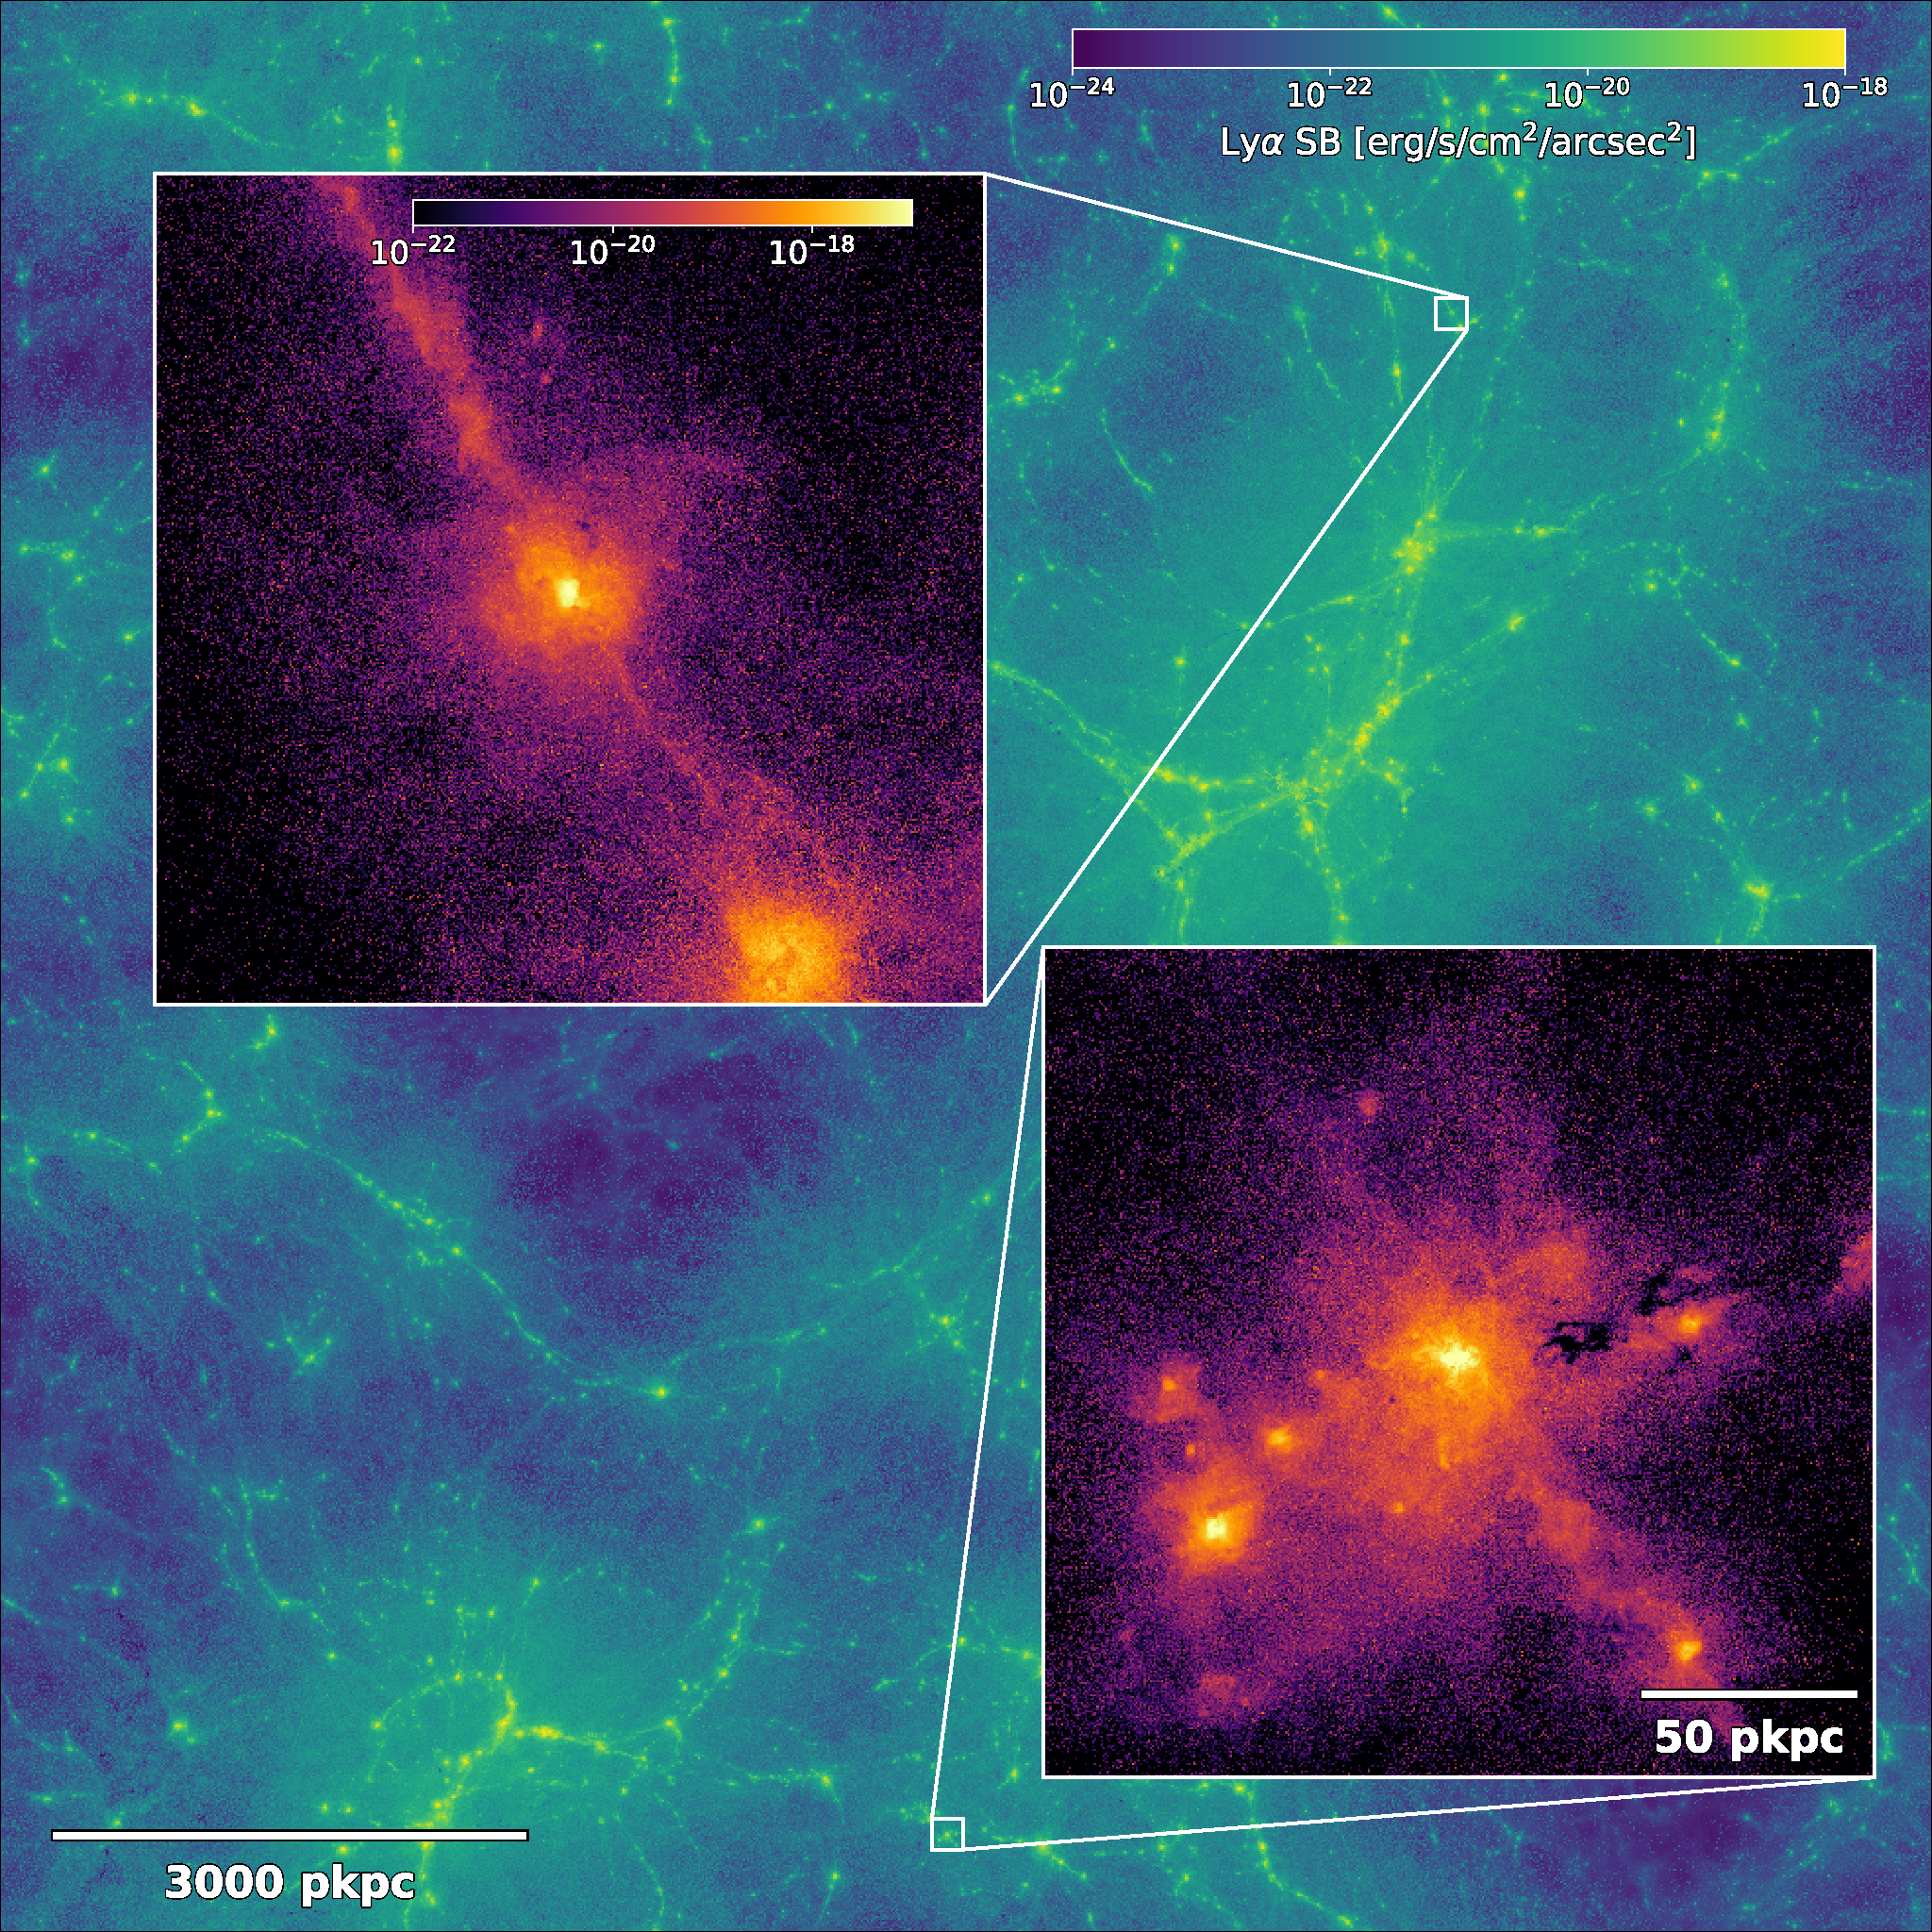
\includegraphics[width=0.7\linewidth]{./pic/TNG50_z3_LymanAlpha_emission_2k.png}
	\caption{}
	\label{fig:TNG50_z3_LymanAlpha_emission_2k}
\end{figure}

Illustrisプロジェクトのシミュレーションを含め,Illustris-TNGプロジェクトのシミュレーションデータは以下の通りが公開されている.

\begin{figure}[H]
	\centering
	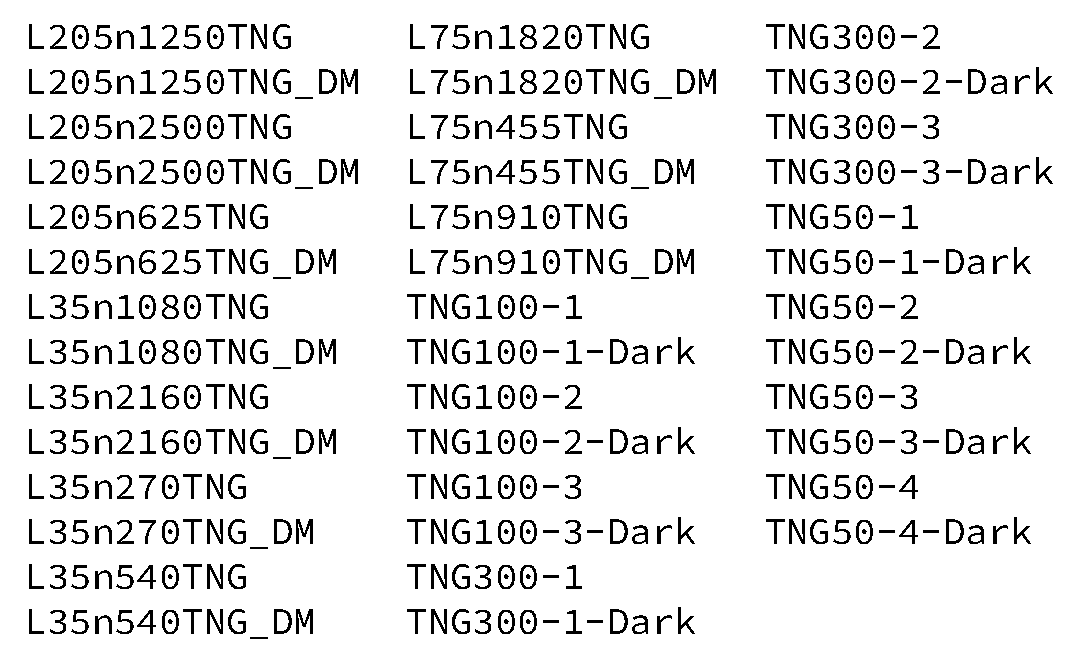
\includegraphics[width=0.5\linewidth]{./pic/ALLsimTNG.pdf}
\end{figure}

シミュレーションデータのディレクトリ下には次のようなディレクトリとファイルが存在する:\texttt{output/},\texttt{processing/},\texttt{simulation.hdf5}

\texttt{output/}ディレクトリ下には,グループカタログ,スナップショット,Subboxなどのデータが存在する.グループカタログにはHalo(銀河団)カタログやSubhalo(銀河)カタログが存在する.スナップショットには宇宙誕生を0として,現在を99として100個のスナップショットファイルが存在する.例えばTNG50-1の場合,宇宙誕生から0.179 Gyrをスナップショット0として13.803 Gyrをスナップショット99としている.ディレクトリ「\texttt{groups\_*}」,「\texttt{snapdir\_*}」の\texttt{*}には3桁でスナップショット番号が入る.現在の宇宙(スナップショット99)を使用したい場合は,ディレクトリ「\texttt{groups\_099}」,「\texttt{snapdir\_099}」を見れば良い.

そのディレクトリ下には,グループカタログやスナップショットのデータは大きいため,複数のファイルに分割されていて,これをチャンクファイルという. グループカタログのチャンクファイルは「\texttt{fof\_subhalo\_tab\_*}」もしくは「\texttt{groups\_*}」のファイル名でで定義され連番表記されている.

\section{face-onとedge-onの導出}
図\ref{fig:faceon,edge-on}のように、銀河の回転面の上方または下方から見ているとき、その銀河をface-on galaxyと呼び、銀河の回転面を横から見ているとき、その銀河をedge-on galaxyという。シミュレーション上に作られた銀河は任意の方向から見ることができ、回転も自由に行うことができる。

\begin{figure}[htbp]
	\centering
	\begin{minipage}[b]{0.48\linewidth}
		\centering
		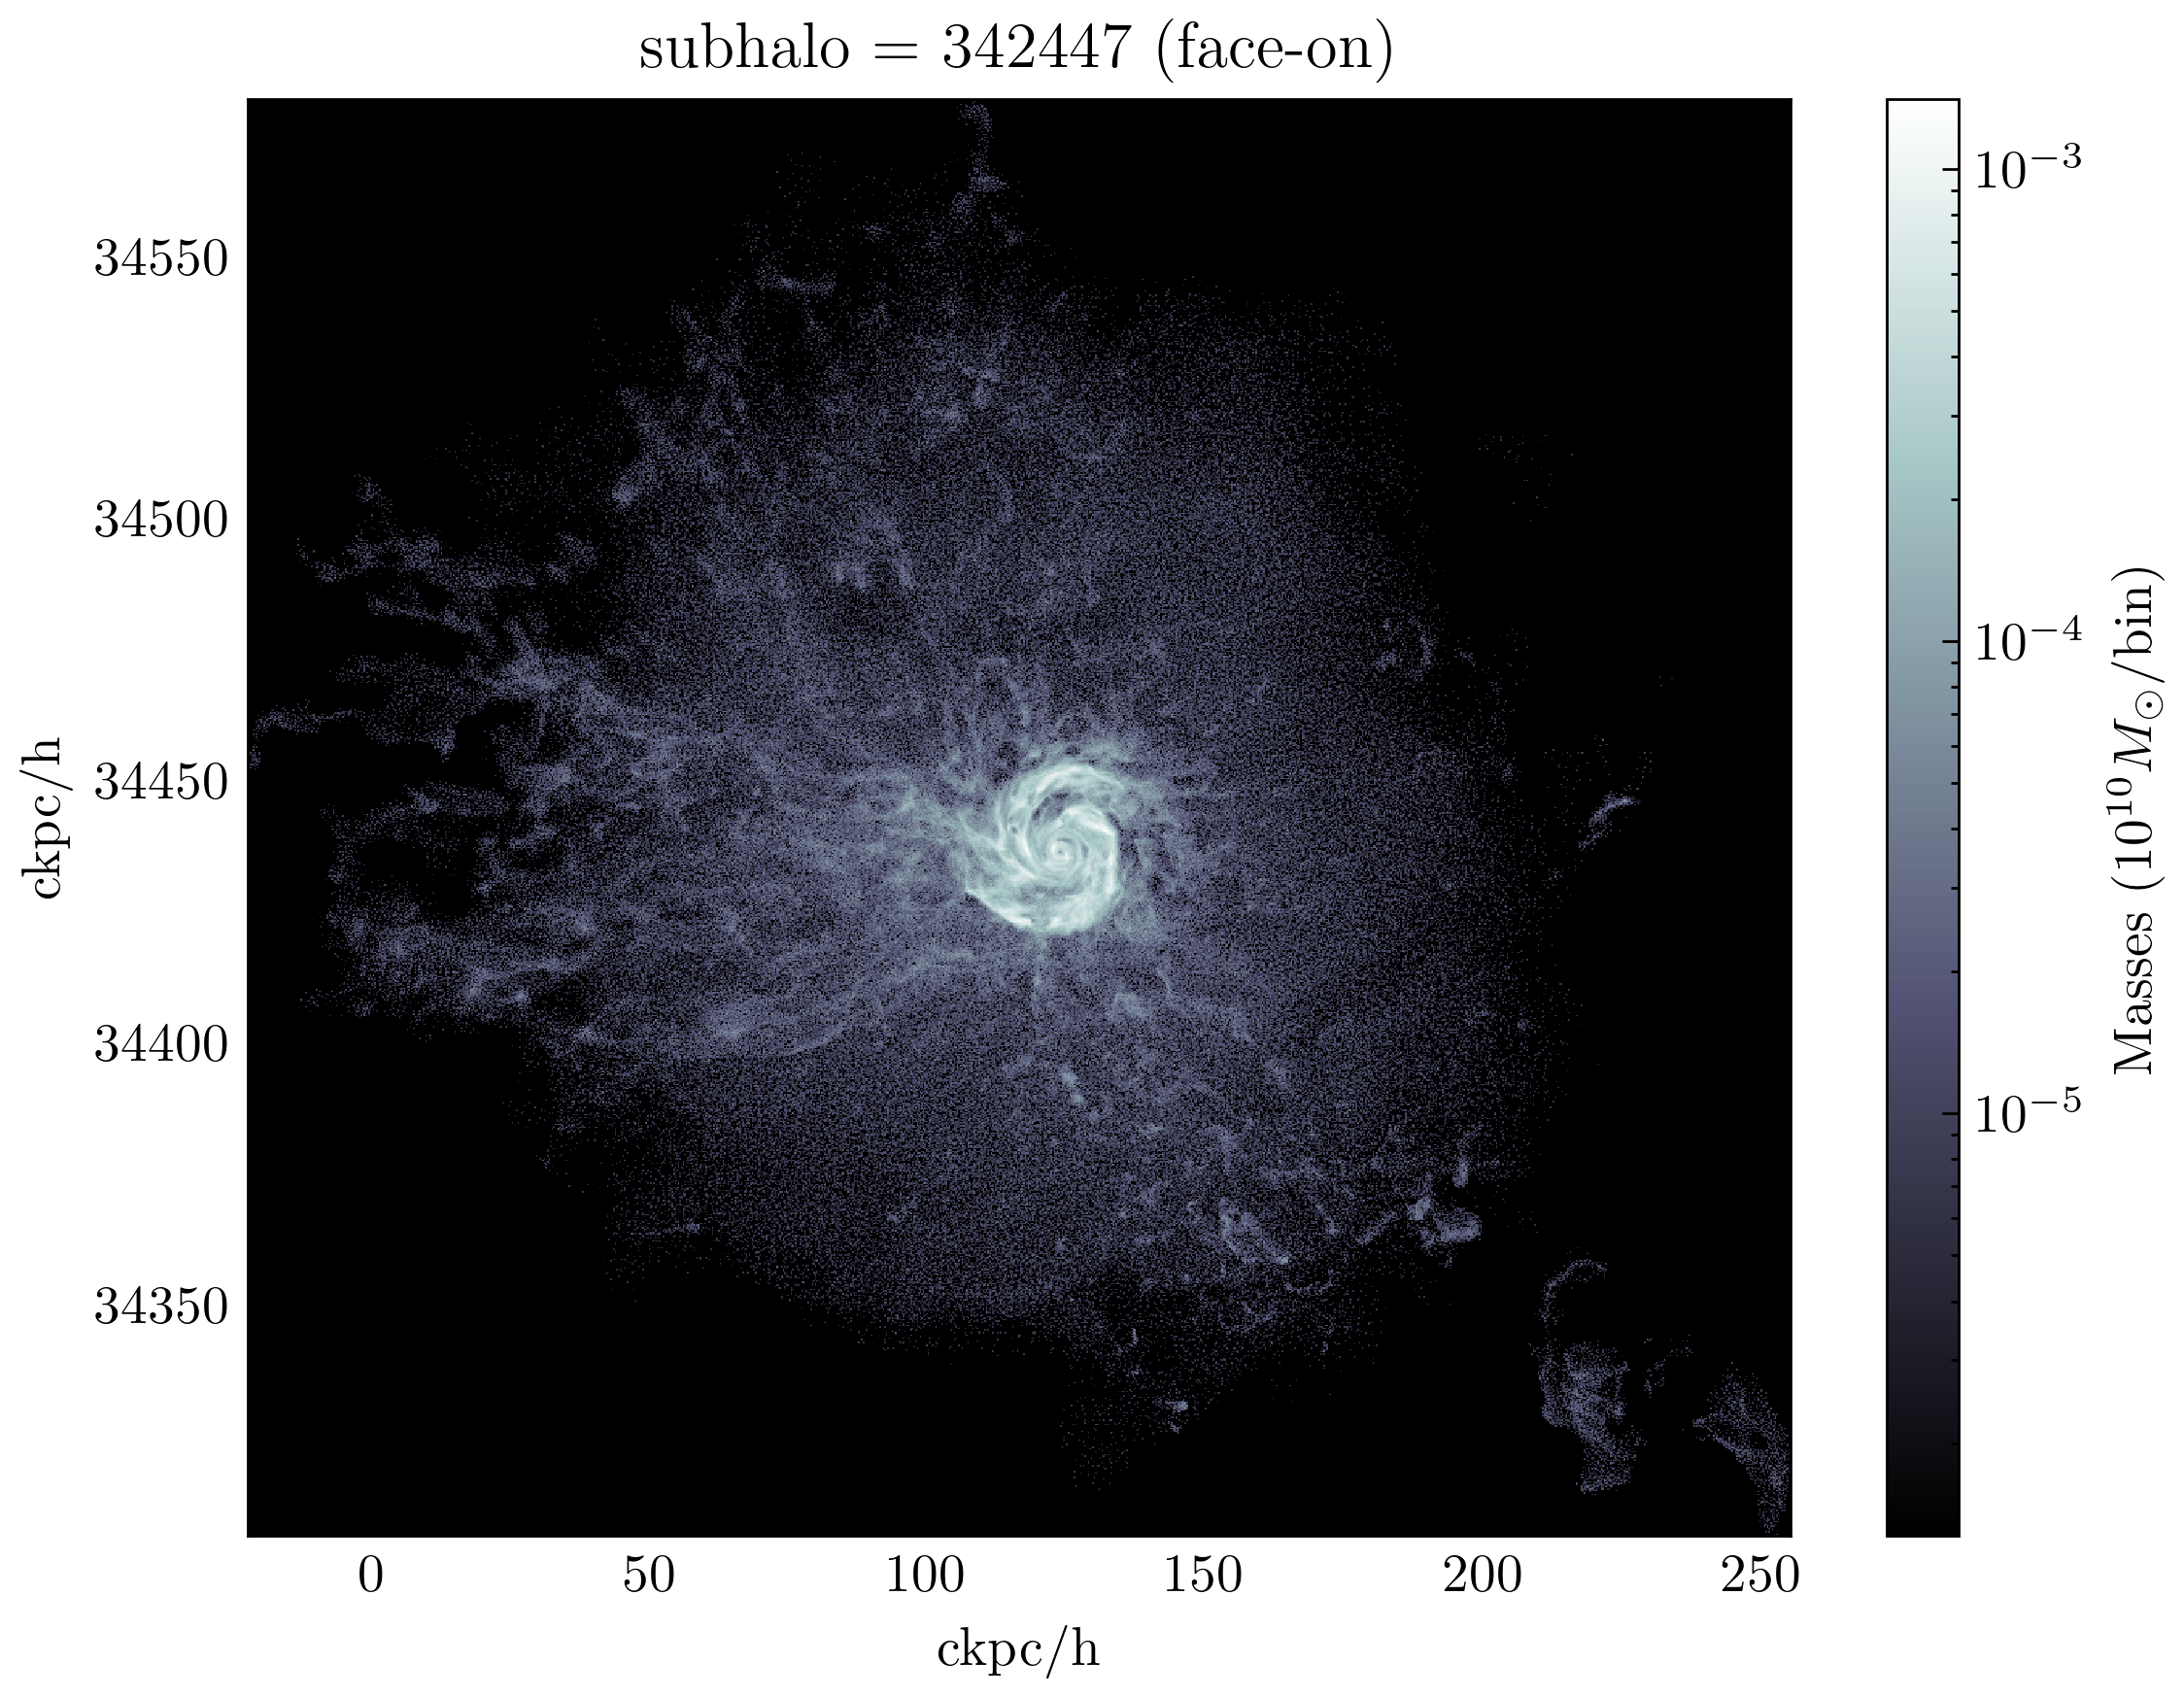
\includegraphics[width=\linewidth]{./pic/face-on}
	\end{minipage}
	\begin{minipage}[b]{0.48\linewidth}
		\centering
		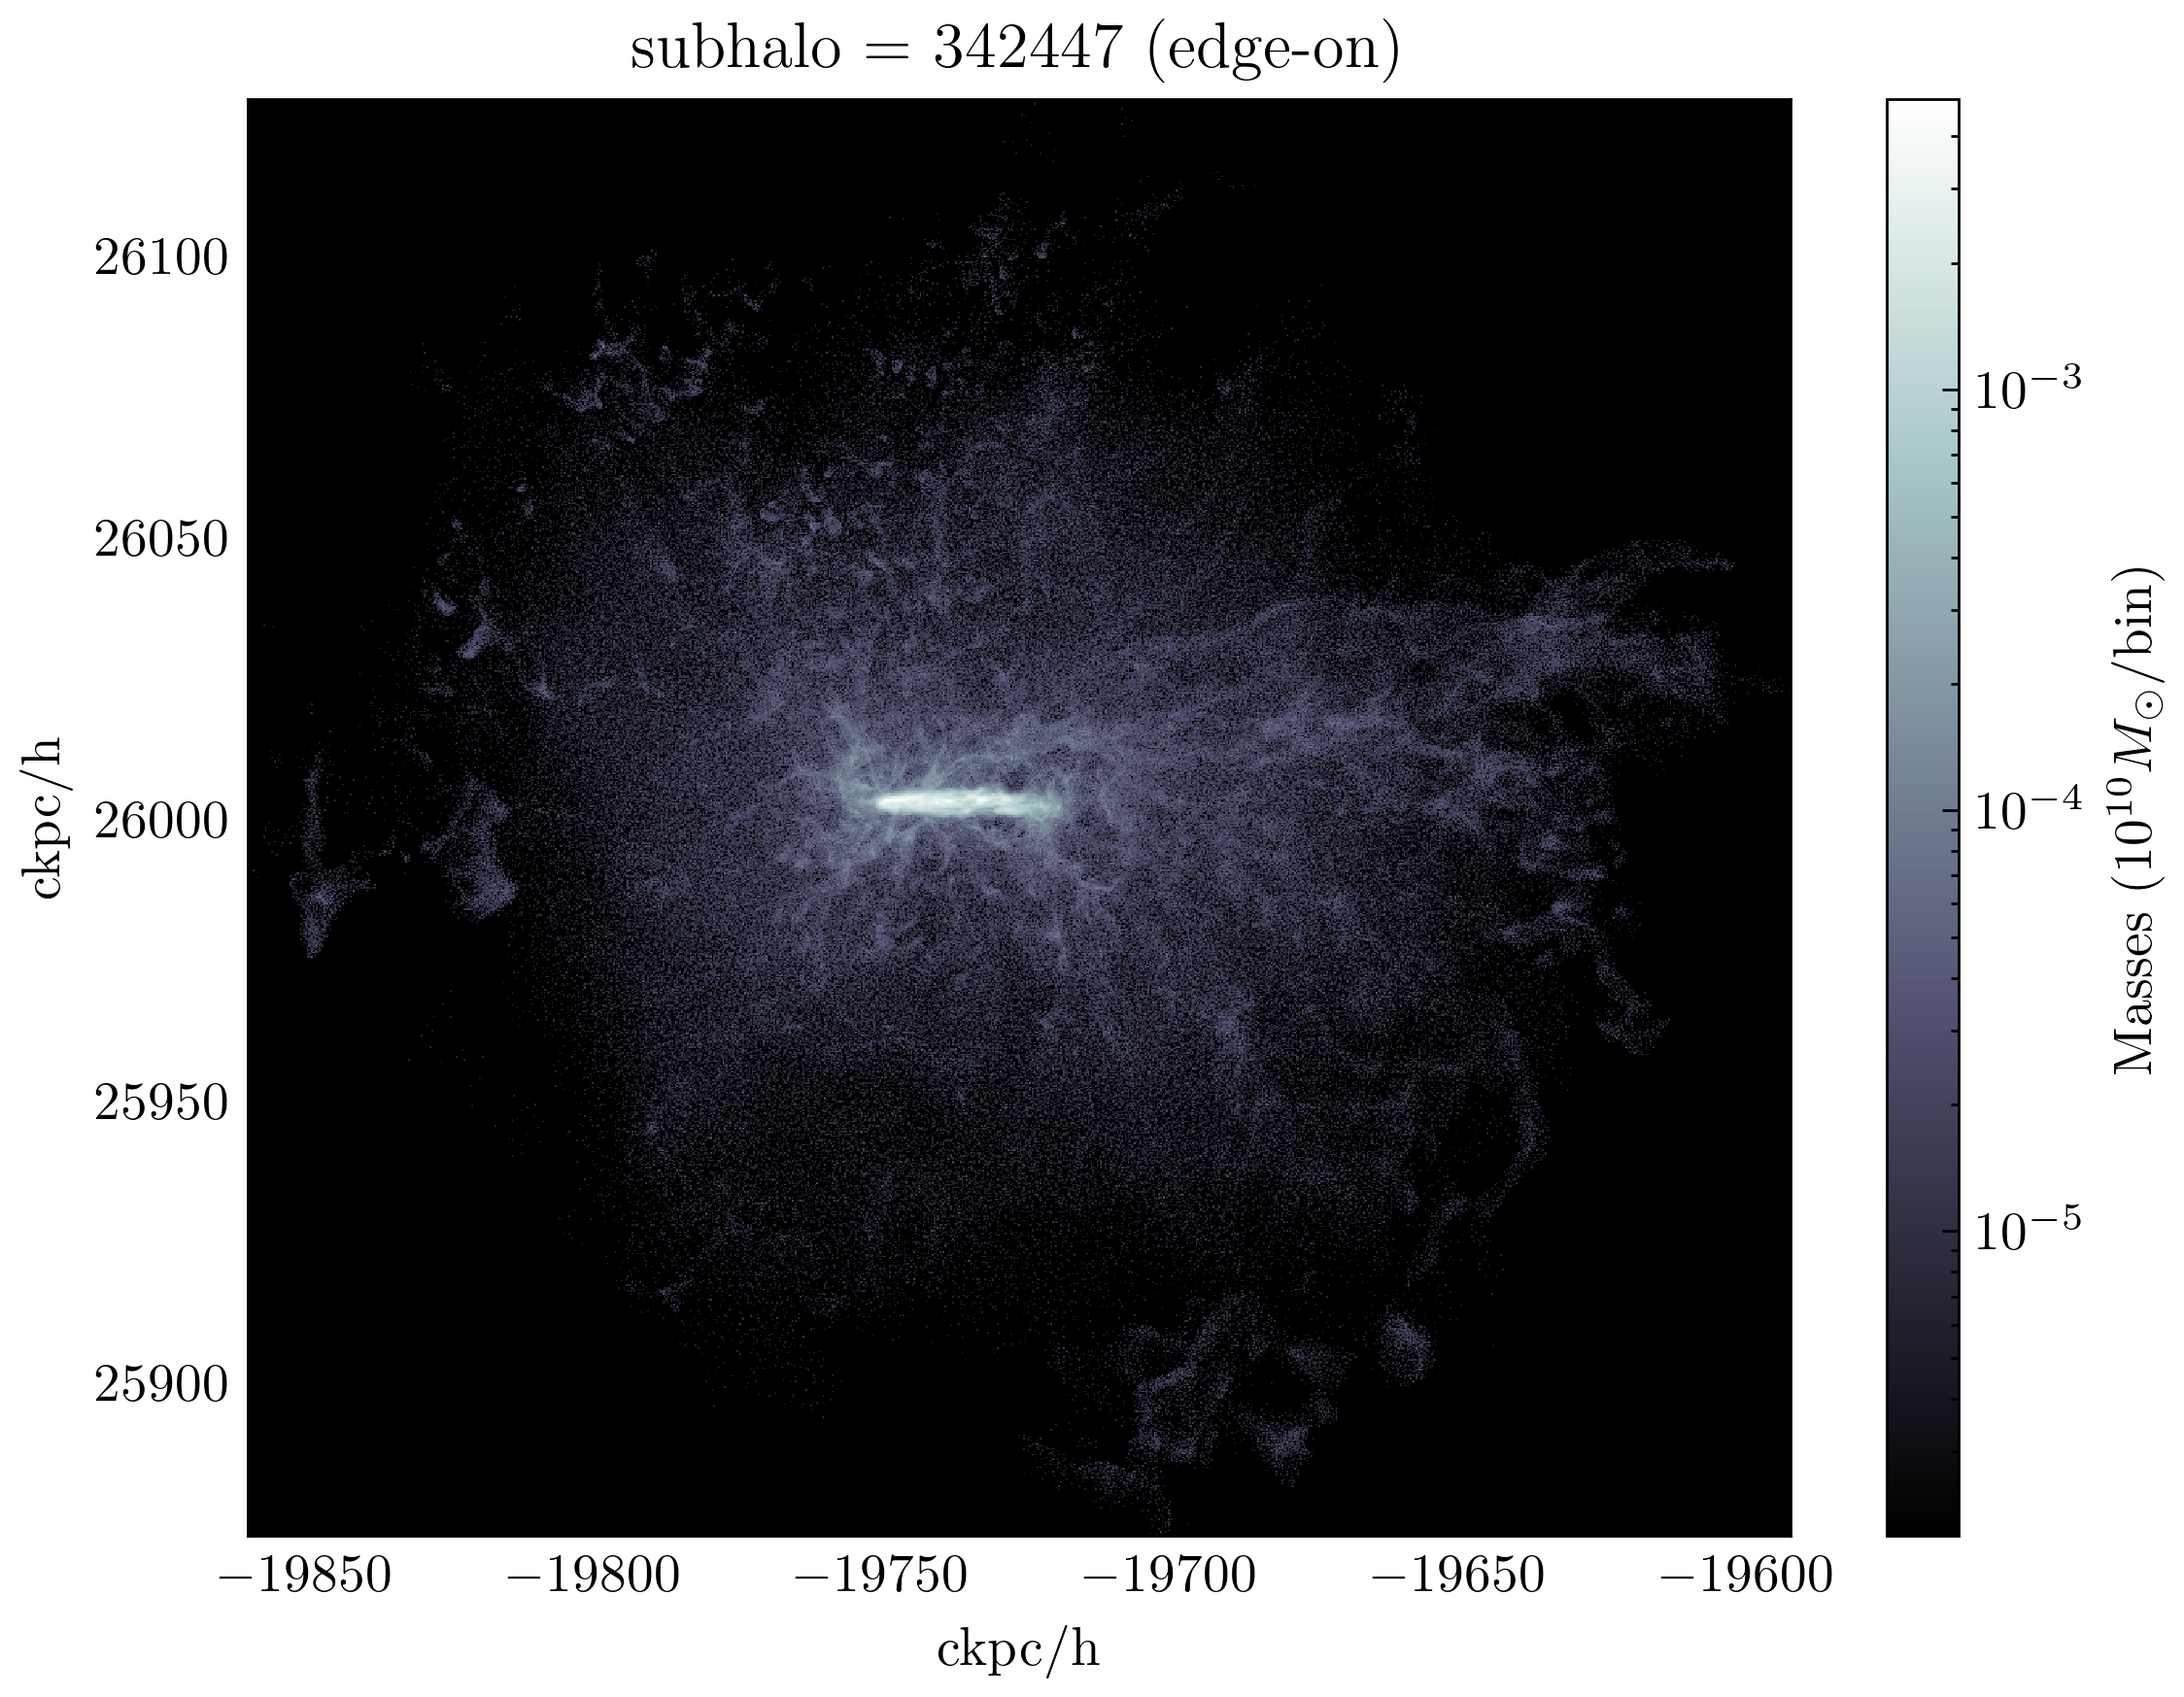
\includegraphics[width=\linewidth]{./pic/edge-on}
	\end{minipage}
	\caption{}
	\label{fig:faceon,edge-on}
\end{figure}

face-onの方向は質量分布が最も安定する方向と見ることもでき、その向きへの回転行列は次のように計算を行うことができる。粒子$i$の座標$(x,y,z)$・質量$m$を添字$i$を用いて慣性モーメントテンソル$I$は
\begin{align}
	I = \sum_{i} \begin{pmatrix}
		m_i (y_i^2 + z_i^2) & -m_iy_ix_i & -m_iz_ix_i \\
		-m_i x_i y_i & m_i (x_i^2 + z_i^2) & -m_i z_iy_i \\
		-m_i x_i z_i & -m_i y_i z_i & m_i (x_i^2 + y_i^2)
	\end{pmatrix}
\end{align}
で与えられる。慣性モーメント$I$の固有値$\lambda_j$ (ただし $\lambda_0 < \lambda_1 < \lambda_2$)、固有ベクトル$\bm{\chi}_j \ (j = 0,1,2)$を求めると、回転行列は$[ \bm{\chi}_0, \bm{\chi}_1, \bm{\chi}_2 ]$となる。またedge-onはさらに$x$軸に対して$\ang{90}$回転すればよい。
\section{ビリアル半径 $R_\text{vir}$}

赤方偏移$z$においてビリアル平衡に達したダークマターハローの平均密度は:
\begin{align}
	\rho_\text{vir}(z) &= \rho_\text{cr} \Delta_\text{vir} \\
	&\simeq \num{1.8e-27} \left( \frac{\Delta_\text{vir}}{200}\right) \left(\frac{h}{0.7}\right)^2 E^2(z) \ \si{g. cm^{-3}}
\end{align}
と表せる。

ここでビリアル半径内の全質量(ビリアル質量)を$M_\text{vir}$を用いると
\begin{align}
	R_\text{vir} &= \left( \frac{3 M_\text{vir}}{4 \pi \rho_\text{vir}(z)} \right)^{1/3} \\
	&\simeq 2.1 \left( \frac{M_\text{vir}}{10^{15} M_\odot} \right)^{1/3} \left( \frac{\Delta_\text{vir}}{200} \right)^{-1/3} \left( \frac{h}{0.7} \right)^{-2/3} E^{-2/3}(z) \quad \si{Mpc}
\end{align}
となり、観測される銀河団のサイズと質量等の関係を近似的に再現する。

ここでは近傍宇宙を考えているので、$z=0$では$E(z) = 1$であり、$\Delta_\text{vir} = 200$のときのビリアル半径を$R_{200}$とすると次の式が成り立つ:
\begin{align}
	R_{200} \simeq 2.1 \left( \frac{M_\text{vir}}{10^{15} M_\odot} \right)^{1/3} \left( \frac{h}{0.7} \right)^{-2/3} \quad \si{Mpc}
\end{align}


%\begin{algorithmic}
%	\Function{Solve\_Virial\_Mass}{$\text{radius}, \text{mass}, \text{density\_DM}, \text{density\_total}$}
%	\State $\text{valid\_indices} \gets \text{indices of } \text{radius} \text{ where } \text{total\_mass} \text{ is not } \infty$
%	\State $\text{radius} \gets \text{radius}[ \text{valid\_indices}]$
%	\State $\text{total\_mass} \gets \text{total\_mass}[ \text{valid\_indices}]$
%	
%	\State $\text{sorted\_radius}, \ \text{sorted\_total\_mass} \gets \text{sort } \text{radius}, \ \text{total\_mass} \text{ based on } \text{radius}$
%	
%	\State $\text{cum\_mass} \gets \text{cumulative sum of } \text{sorted\_total\_mass}$
%	
%	\State $h \gets 0.6774$
%	
%	\State $\text{virial\_radius} \gets 2.1 \times \left(\frac{\text{cum\_mass} \times 10^{10}}{10^{15}}\right)^{\frac{1}{3}} \times \left(\frac{h}{0.7}\right)^{-\frac{2}{3}}$
%	
%	\State $\text{min\_index} \gets \text{index of the element in } \text{radius}$ \\
%	\qquad \qquad \qquad \qquad \qquad$\text{ with the smallest value of } (\text{radius} - \text{virial\_radius})^2$
%	\State $ r_{200} \gets \text{radius}[\text{min\_index}]$
%	
%	\State \textbf{return} $r_{200}$
%	\EndFunction
%\end{algorithmic}
\section{outflowの計算}
    \documentclass[main.tex]{subfiles}
\begin{document}
	\chapter{結果}
\end{document}

    \documentclass[main.tex]{subfiles}
\begin{document}
	\chapter{議論}
	\section{subhalo342447における$\mathrm{[X/Fe]} > 0$について}

図\ref{fig:fe10}に示すように,X $=$ Ne, O, Mg, Siとして$\mathrm{[X/Fe]} > 0$がいえる.このようなXをアルファ($\alpha$)元素という.中性子数と陽子数が偶数で等しく,$\alpha$粒子(\ce{^{4}He})の集まりと見なせることから,この名前で呼ばれている.Feよりもアルファ($\alpha$)元素が多いということは,アルファ($\alpha$)元素の生成元される重力崩壊型超新星爆発(II型超新星爆発)に由来するものと考えられる.

II型超新星の中心部では核融合反応が進行し,アルファ($\alpha$)元素を生成する.核融合のエネルギーと重力が平衡状態であったのが,鉄まで生成されると平衡状態が崩れ,収縮を始める.中心核は中性子の縮退圧と重力が枯渇すると急停止し,上層は中心核によって反跳し衝撃波が発生する.ゆえに大量のアルファ($\alpha$)元素を宇宙空間にばらまくことになる.

\section{アウトフローと太陽組成比との関係}

アウトフローが観測されたsubhalo342447は図\ref{fig:abundanceprofile342447}に示したように,R/R$_{200} < 0.1$において太陽組成の2倍近くFe, O, Mg, Siなどの元素が観測された.一方でアウトフローが観測されなかったsubhalo388544やsubhalo421555はR/R$_{200} < 0.1$において太陽組成程度であることが観測された(図\ref{fig:2radicalprofile}).

このようなことからアウトフローと太陽組成には何らかの因果関係がある可能性がある.

\section{subhalo342447の「へこみ」と温度分布の高温部}

図\ref{fig:fe10}において$0.1<\text{R/R}_{200} < 0.5$で他の部分と組成が異なる「へこみ」が観測されたことに加え,図\ref{fig:atemp}の右側で,R/R$_{200} < 0.1$においては\SI{e6}{K}以上の高温ガスが確認できたことから,subhalo342447が現在の状態になるまでに,他のsubhaloと衝突をし,そのsubhaloの組成の一部を取り込んだ可能性が考えられる.

\begin{figure}[htbp]
	\centering
	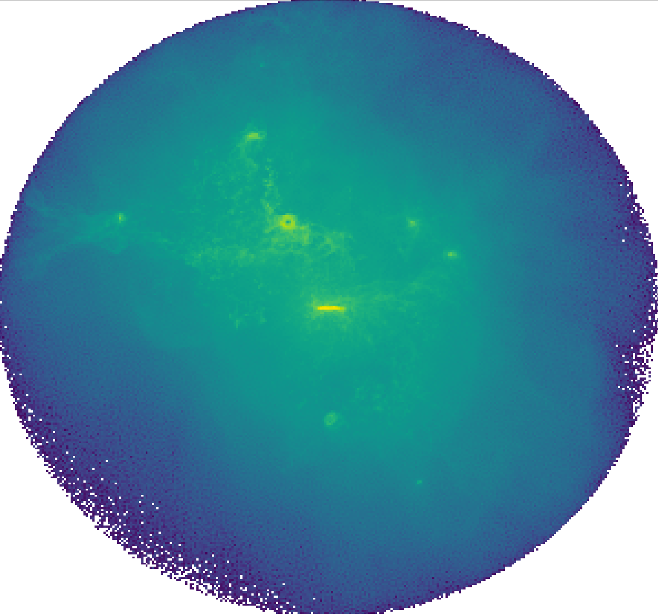
\includegraphics[width=0.6\linewidth]{pic/virial3}
	\captionsetup{width=0.9\linewidth}
	\caption{subhalo342447をedge-onにした状態で中心にとり,ビリアル半径の3倍を表示.濃淡は対数で質量を表す.}
	\label{fig:virial3}
\end{figure}

また図\ref{fig:virial3}に示すようにsubhalo342447の周囲に別のsubhaloが観測され,ガスの散乱具合も衝突後のような状態となっている.このようなことから衝突した可能性は非常に高いと考えられる.
\end{document}
    \chapter{まとめ}
    \chapter*{謝辞}
\addcontentsline{toc}{chapter}{謝辞}


    
    \nocite{*}
    \bibliographystyle{aasjournal}
    \bibliography{res2023}
    \addcontentsline{toc}{chapter}{\bibname}
    
\end{document}